\chapter{Wind Turbine Monitoring} \label{s:wt_monitoring}
% First give a short summary of the spectra of different condition monitoring schemes. Importance of predictive maintainance, and \textbf{short summary} of current implementations of predictive maintainance schemes. 

\section{Wind turbine Components}
% Introduce the basic components of a wind turbine, and present some fun statistics about when the different components fail. 
\begin{figure}[h]
    \begin{center}
    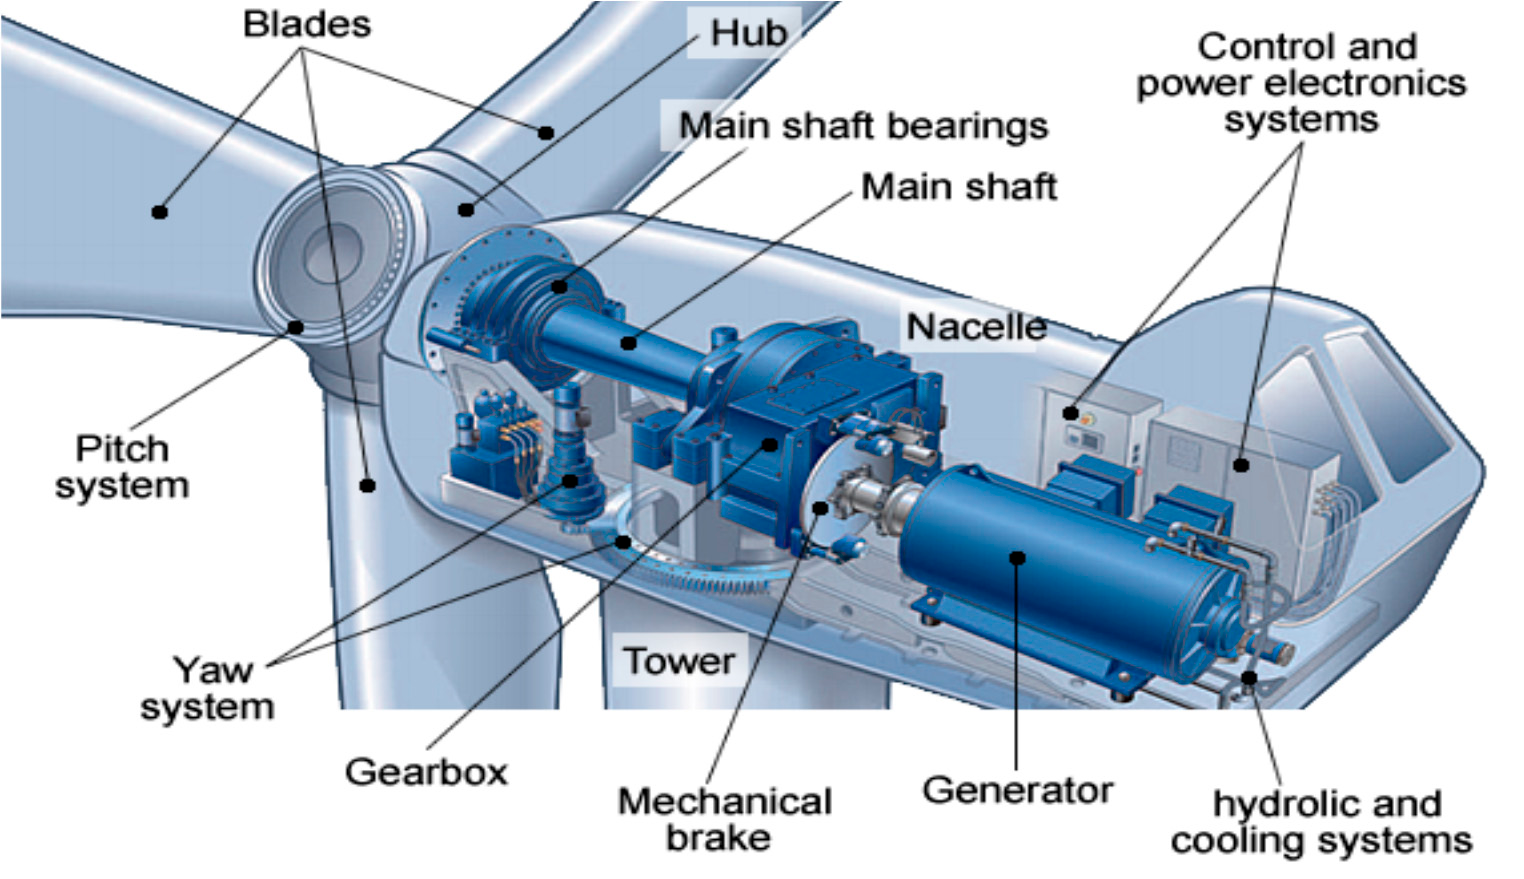
\includegraphics[width=0.8\textwidth]{wind_turbine/wt_parts.png}
    \end{center}
    \caption{Illustration of the different parts of a wind turbine, taken from \cite{adv_meth_for_wt_cond_monit_rev}}
    \label{fig:wt_parts}
\end{figure}

Figure \ref{fig:wt_parts} shows the main parts of a wind turbine which includes the rotor (blades and hub), shafts, gearbox and generator. Simplified a wind turbine works by wind pushing the blades, generating torque that makes the hub rotate. The hub is connected to the gearbox through the main shaft. The gearbox then gears down the torque and gears up the rotational speed to a level that the generator can use to induce current, that goes to a station that transforms the voltage to a level that can be used in the electrical grid. 

\section{Sensors and Data Acquisition}

Information about a wind turbine can come from many sources, it can come from external sources such as images from a camera, or from internal sensors measuring operational data. The collective term for systems measuring operational data is supervisory control and data acquisition (SCADA) systems. To choose what algorithm to use, or what model to use, one must first consider what data one has available. From the literature considered, these where the most used forms of data used as input for the model. 

\begin{itemize}
    \item Vibration measurement  %\cite{wt_bearing_cm_review} \cite{wt_cm_rev_new_trends_chal_2014}
    \item Acustic emission monitoring %\cite{wt_bearing_cm_review} \cite{wt_cm_rev_new_trends_chal_2014}
    \item Temperature measurement %\cite{wt_bearing_cm_review} \cite{wt_cm_rev_new_trends_chal_2014}
    \item Power signal measurement %\cite{wt_bearing_cm_review} \cite{wt_cm_rev_new_trends_chal_2014}
    \item Oil debris monitoring %\cite{wt_bearing_cm_review} \cite{wt_cm_rev_new_trends_chal_2014}
    \item Strain monitoring %\cite{wt_cm_rev_new_trends_chal_2014}
    \item Optical fiber monitoring %\cite{wt_cm_rev_new_trends_chal_2014}
    \item Ultrasonic testing %\cite{wt_cm_rev_new_trends_chal_2014}
    \item Image analysis
\end{itemize}

Analysis of vibration signals is the most common form of condition monitoring used in industry for any form of rotating equipment \cite{wt_bearing_cm_review}. By measuring the acustic emission generated by a component of a wind turbine, one can estimate how much damage it has obtained. The temperature of components in a wind turbine is closely correlated with the health of the component, and is therefore used often in condition monitoring applications \cite{DBN_chicken_swarm_optim}. The power signal can also say a lot about how well a wind turbine is performing, specifically the wind speed - power curve. When monitoring the debris in the oil of a wind turbine gearbox one is analysing the size, type and number of wear particles present in the lubricant, as they can indicate the degree of damage in the gearbox \cite{cm_rnn_lstm}. Strain monitoring, optical fiber monitoring, ultrasonic testing, and image analysis are all used to detect structural damage in different components of the wind turbine, usually the blades \cite{lin_and_non_lin_feat_for_ice_detection_on_blades, image_based_surface_damage_detection_DL_drone_inspection,image_based_YOLO_YSODA, dirt_n_mud_detection_using_guided_waves,blade_defect_detection_imaging_array, unsupervised_AD_blade_damage_deep_features_images}, or tower \cite{wt_cm_rev_new_trends_chal_2014}. The most common approach however was to use a combination of multiple sensors-values to make predictions about the condition about the wind turbine.

\section{Machine learning techniques}
A machine learning is a subset of artificial intelligence. Machine learning models that extract rules from data, which can then be applied to classify, or estimate components of another dataset. Machine learning algorithms are formally divided into \textit{supervised learning}, \textit{unsupervised learning} and \textit{semi-supervised learning}. Supervised learning models require labelled datasets to extract information from the dataset, and are usually used to perform classification tasks, or to estimate a variable that is considered dependent on the input variables (regression). Unsupervised learning algorithms do not require labelled datasets. Semi-supervised learning uses a combination of labelled and unlabelled datasets. \bigskip

\subsection{Feature extraction}
There are two central problems in condition monitoring that can be solved by feature extraction and selection. The first is the sheer volume of information being produced. A wind turbine with only 20 sensors, sampled at 100 Hz will produce 170 MB of information per day. Feature selection is used here to reduce the number of features to only those relevant for condition monitoring. The second problem is that for systems using only one signal such as vibration, there are many components that are superposed to create the measured signal, and noise is present. Feature extraction is used to separate the interesting components from each other, and cancel the noise. For some machine learning models feature extraction is not a neccesary preprocessing step, for others careful though must be given as to how to extract features. Table \ref{tab:feat_ext_wt} shows the most frequent methods found in the articles. 

\begin{table*}
    \centering
    \ra{1.3}
    \begin{tabular}{p{0.31\textwidth}p{0.3\textwidth}}
        \toprule
        Extraction method                   & Articles \\
        \midrule
        ARMA models                         & \cite{ml_cm_wt_blade_ARMA_2018, fault_detection_and_isolation_using_classifier_fusion, lin_and_non_lin_feat_for_ice_detection_on_blades, dirt_n_mud_detection_using_guided_waves, vibration_ARMA_decision_tree_cm_wt} \\
        Discrete Wavelet Transform (DWT)    & \cite{fault_detection_and_isolation_using_classifier_fusion, image_texture_analysis_FD_wt, vibration_acustic_decision_tree_SVM_gearbox, integrated_cm_bearing_fault_wt_gearbox} \\
        Principal Component analysis (PCA)  & \cite{lin_and_non_lin_feat_for_ice_detection_on_blades, multiway_PCA_multivar_inference_cm_wt, dirt_n_mud_detection_using_guided_waves, integrated_cm_bearing_fault_wt_gearbox, unsupervised_AD_blade_damage_deep_features_images, online_fd_using_PCA_different_operating_zones, fault_detect_PARAFAC_k_means}\\
        Basic signal statistics             & \cite{blade_damage_detection_sup_ml_alg, integrated_cm_bearing_fault_wt_gearbox, roller_bearings_cm_fisher_score_and_permutation_entropy} \\
        \bottomrule
    \end{tabular}
    \caption{Feature extraction methods}
    \label{tab:feat_ext_wt}
\end{table*}

The DWT is a method used for decomposing time-dependent signals. It is a better alternative than other time-frequency decomposition tools, such as the Fourier transform (FT), for non-stationary signals. However, the FT is also used \cite{fault_detection_and_isolation_using_classifier_fusion, blade_damage_detection_sup_ml_alg}. Basic signal statistics refers to values easy to calculate over a fixed window size such as the root-mean-square (RMS) value, min/max value, etc. PCA is an unsupervised machine learning form used in multivariate systems. It produces the linear combinations of variables that has the highest variance, also called the \textit{principal components}. \newpage

% NN, especially convolutional neural networks (CNN) have been found useful for object detection in images, as done by \textcite{image_based_surface_damage_detection_DL_drone_inspection, unsupervised_AD_blade_damage_deep_features_images} for detecting defects in the wind turbine blades. \textcite{ice_detection_using_ITL} and \textcite{VMD_MPE_COVAL_fault_detection_gearbox} use NN for transfer learning. 

\subsection{Regression-based models}
A frequent approach is to use a supervised learning model to capture the normal behaviour of a wind turbine (or wind turbine component) by predicting the value of one time dependent variable, and then using the deviation between the prediction and the actual value (Estimation error $E_e$) to detect anomalous behaviour. What varies in these approaches is what machine learning model they use to model the wind turbine. The input data used in this approach is most often SCADA data. The target variable is either a particular signal which is excluded from the input signals, or the target is to recreate the input signal as accurately as possible. The latter approach is called an \textit{auto-encoder}. Three curves in particular hold a lot of information about the performance of a wind turbine, namely the wind speed - active power curve, wind speed - rotor speed curve and wind speed - blade angle pitch curve. The majority of the regression based models, used a subset of these curves as target variables \cite{perf_mon_of_wt_using_extreme_func_theory, GP_operational_curve_monitoring, high_freq_scada_perf_monit_sensitivity, abnormal_detection_scada_data_mining, improved_power_curve_monitoring_of_wt, SVR_blade_pitch_curve_cm, health_cond_model_nn_proportional_hazard_models}. Another popular approach is to forecast the temperature in the gearbox, or generator windings \cite{AD_and_fault_analysis_wt_DAE, health_cond_model_nn_proportional_hazard_models, detecting_malfunctions_wt_generator_bearings_generic_vs_specific_models, CBPM_ABPM_maintainance_model, wt_gearbox_bearing_temp_KS_CNN, DBN_chicken_swarm_optim}. As mentioned before temperature is closely correlated with the health of a component, but since temperature changes so slowly it is hard to use temperature monitoring alone for fault prediction \cite{wt_cm_rev_new_trends_chal_2014}. If one however can make a model capture the complex sources of temperature change, the deviation between predicted temperature, and actual temperature could be used for fault prediction. Table \ref{tab:regression_ml_models} shows the typical machine learning models used for regression. 

% \begin{table*}[h]
%     \centering
%     \ra{1.3}
%     \begin{tabular}{p{0.35\textwidth}p{0.3\textwidth}}
%         \toprule
%         Target variable               & Articles \\
%         \midrule
%         Power curve                   & \cite{perf_mon_of_wt_using_extreme_func_theory, GP_operational_curve_monitoring, high_freq_scada_perf_monit_sensitivity, abnormal_detection_scada_data_mining, improved_power_curve_monitoring_of_wt} \\
%         Blade pitch curve             & \cite{GP_operational_curve_monitoring, abnormal_detection_scada_data_mining, SVR_blade_pitch_curve_cm} \\
%         Vibration signal              & \cite{ANN_damage_detection_gearbox_wt} \\
%         Rotor speed curve             & \cite{GP_operational_curve_monitoring, abnormal_detection_scada_data_mining, health_cond_model_nn_proportional_hazard_models} \\
%         Gearbox/generator temperature & \cite{AD_and_fault_analysis_wt_DAE, health_cond_model_nn_proportional_hazard_models, detecting_malfunctions_wt_generator_bearings_generic_vs_specific_models, CBPM_ABPM_maintainance_model, wt_gearbox_bearing_temp_KS_CNN} \\
%         Reproduce input               & \cite{auto_associative_nn_wt_fault_detection, DBN_simulink_SCADA_FD} \\
%         High speed shaft              & \cite{CBPM_ABPM_maintainance_model} \\
%         \bottomrule
%     \end{tabular}
%     \caption{Target variables used for normal behaviour modelling}
%     \label{tab:target_variables}
% \end{table*}

\begin{table*}[h]
    \centering
    \ra{1.3}
    \begin{tabular}{p{0.45\textwidth}p{0.3\textwidth}}
        \toprule
        Machine learning model                          & Articles \\
        \midrule
        Neural networks (NNs)                           & \cite{improved_power_curve_monitoring_of_wt, ANN_damage_detection_gearbox_wt, health_cond_model_nn_proportional_hazard_models, detecting_malfunctions_wt_generator_bearings_generic_vs_specific_models, CBPM_ABPM_maintainance_model, wt_gearbox_bearing_temp_KS_CNN, auto_associative_nn_wt_fault_detection} \\
        Gaussian process (GP) regression                & \cite{perf_mon_of_wt_using_extreme_func_theory, GP_operational_curve_monitoring} \\
        Support vector regression (SVR)                 & \cite{high_freq_scada_perf_monit_sensitivity, abnormal_detection_scada_data_mining, SVR_blade_pitch_curve_cm} \\
        PCA                                             & \cite{online_fd_using_PCA_different_operating_zones} \\
        K-nearest neighbours (KNN)                      & \cite{high_freq_scada_perf_monit_sensitivity} \\
        Random forest (RF)                              & \cite{high_freq_scada_perf_monit_sensitivity} \\
        Network of restricted Boltzman machines (RBMs)  & \cite{AD_and_fault_analysis_wt_DAE, DBN_chicken_swarm_optim} \\
        \bottomrule
    \end{tabular}
    \caption{Machine learning algorithms used by normal behaviour models}
    \label{tab:regression_ml_models}
\end{table*}

%% NN
% Artificial NNs are hereby referred to as NNs. They are composed of layers of artificial neurons known as \textit{perceptrons}. Single perceptrons can only capture linear relationships between input variables, and by combining multiple layers containing many perceptrons, together with non-linear activation functions, NN are able to capture complex non-linear relationships between variables, and are therefore a popular choice as regression model. By the addition of convolutional layers to a NN, they are better able to reduce the dimensions of high dimensional data, and by using layers with a feedback function (recurrent layers) NN become better at capturing long-term time dependent features.

%% Comparison
\textcite{ANN_damage_detection_gearbox_wt} train a NN to estimate the vibration in a gearbox using gearbox oil temperature, wind speed, rotor speed and active power as an input. By performing linear regression on the estimation error of the NN they are able to detect early states of damage in a gearbox, months before it is replaced. \textcite{detecting_malfunctions_wt_generator_bearings_generic_vs_specific_models} compare different NN using SCADA data from 14 wind turbines monitored over several years, trained to estimate the temperature of the bearing on the non-drive end of a generator. They are able to detect failueres within 2 months of occurance. \textcite{health_cond_model_nn_proportional_hazard_models} propose a model of three different NN that estimate the rotor speed, gearbox temperature, and generator winding temperature using SCADA data. The estimation error for the NNs are then forwarded to a proportional hazard model which sets a dynamic threshold for anomalous behaviour. NN are by far one of the best models to capture complex non-linear relationships between input variables, and in contrast to the kernel methods such as GP and SVR they are less relient on data being preprocessed, and features being extracted from the data beforehand. Instead what features a NN is able to extract is decided by the size, and complexity of the archtitecture. One of the disadvantes of using NNs is that the require a lot of training data to be accurate compared to other. The amount of training data required by a NN is also decided by the complexity of it's architecture. \textcite{high_freq_scada_perf_monit_sensitivity} chooses not to use NNs in their approach because they are prown to overfitting, instead they compare three other approaches of SVR, KNN and RF to estimate the active power. They found that the RF regressor trained with high frequency SCADA data produced the best results when trained on short periods. \textcite{abnormal_detection_scada_data_mining} use Grey correlation algorithm for eigenvector extraction and genetic algorithms for feature selection and an SVR to estimate all three performance curves. \bigskip

\textcite{DBN_chicken_swarm_optim} use a \textit{Deep Belief Network} (DBN) that consists of two layers of RBMs, and an output layer. It uses the DBN to predict the gearbox main bearing temperature, and sets a threshold for $E_e$ to detect anomalies. \textcite{AD_and_fault_analysis_wt_DAE} also uses a network of RBMs, but use them an auto-encoder, and then uses the reconstruction error $R_e$ to detect an anomaly. DBN have a great potential for both regression and classification tasks, but as with NN their performance is highly dependent on their architecture, and the data used to train them. \textcite{auto_associative_nn_wt_fault_detection} use an auto-associative NN as an auto-encoder, and then use the Hotel $T_2$ statistic as a dynamic threshold for $R_e$. The use of dynamic thresholds is very 

\subsection{Supervised classification-based models}

\begin{table*}[h]
    \centering
    \ra{1.3}
    \begin{tabular}{p{0.45\textwidth}p{0.3\textwidth}}
        \toprule
        Machine learning model & Articles \\
        \midrule
        Neural network based                            & \cite{image_based_surface_damage_detection_DL_drone_inspection, image_based_YOLO_YSODA, AI_image_analytics_2_classify_blade_defects, blade_defect_detection_imaging_array, model_based_fuzzy_logic_cm_wt, deep_learning_for_imbalanced_class_detection_bearing_cm} \\
        Tests several individual classifiers            & \cite{ml_cm_wt_blade_ARMA_2018, lin_and_non_lin_feat_for_ice_detection_on_blades, image_texture_analysis_FD_wt, ice_detection_using_ITL, vibration_ARMA_decision_tree_cm_wt} \\
        Uses fusion / ensamble of classifiers           & \cite{fault_detection_and_isolation_using_classifier_fusion, dirt_n_mud_detection_using_guided_waves, RF_XGB_fault_detection} \\
        Support Vector Classifier (SVC)                 & \cite{blade_damage_detection_sup_ml_alg, VMD_MPE_COVAL_fault_detection_gearbox, vibration_acustic_decision_tree_SVM_gearbox, fault_classification_using_CSO_SVM, integrated_cm_bearing_fault_wt_gearbox, roller_bearings_cm_fisher_score_and_permutation_entropy} \\
        Hierarchical Extreme Learning Machine (H-ELM)   & \cite{wt_cm_using_cloud_computing_and_HELM} \\
        DBN                                             & \cite{DBN_simulink_SCADA_FD} \\ 
        Hidden Markov model (HMM)                       & \cite{fault_monitoring_HMM} \\
        \bottomrule
    \end{tabular}
    \caption{Machine learning algorithms used by supervised classification models}
    \label{tab:sup_classification_ml_models}
\end{table*}

\textcite{image_based_surface_damage_detection_DL_drone_inspection, image_based_YOLO_YSODA, AI_image_analytics_2_classify_blade_defects, blade_defect_detection_imaging_array} use images as input, and different types of NN for classifying structural damage in the blades. \textcite{deep_learning_for_imbalanced_class_detection_bearing_cm} uses SCADA data as input, and deep NN for detecting ice on the blades. The testing, and comparing of several individual classifiers is also quite popular, however the most popular classifier by far is the SVC. The SVC has also been used for detecting damage in the blades \cite{blade_damage_detection_sup_ml_alg}, general fault detection in the turbine \cite{fault_classification_using_CSO_SVM}, but most for gearbox faults \cite{VMD_MPE_COVAL_fault_detection_gearbox,vibration_acustic_decision_tree_SVM_gearbox, integrated_cm_bearing_fault_wt_gearbox, roller_bearings_cm_fisher_score_and_permutation_entropy}. \textcite{fault_monitoring_HMM} use a statistical model based on HMMs. They combine multiple vibration signals measured by a condition monitoring system with thresholds, and set different alarm levels. These alarm levels act as the observations for the HMM. The states of the model are \textit{Normal} and \textit{Fault}. The model is trained with sequences of observations, which it uses to determine which state is most probable of producing said sequence of observations. 

\newpage
\subsection{Unsupervised classification-based models}
The classification models have been split into supervised and unsupervised classifiers because, the unsupervised methods are of greater interest for this review. The use of unsupervised learning methods are not as widespread as the use of supervised learning methods. \textcite{ml_for_wt_cond_monit_rev} only included one article in their review that compared a regression model based on feed forward neural networks to two unsupervised models using gaussian mixture models and self organizing maps. It should be noted that the articles using an unsupervised learning approach that are included in this review, generally were published after \cite{ml_for_wt_cond_monit_rev}.

\begin{table*}[h]
    \centering
    \ra{1.3}
    \begin{tabular}{p{0.45\textwidth}p{0.3\textwidth}}
        \toprule
        Machine learning model & Articles \\
        \midrule
        RBMs                    & \cite{unsup_graphical_modeling_wt_cm} \\
        K-means clustering      & \cite{fault_detect_PARAFAC_k_means} \\
        One-class SVM (OCSVM)   & \cite{unsupervised_AD_blade_damage_deep_features_images} \\
        Multiway PCA            & \cite{multiway_PCA_multivar_inference_cm_wt} \\
        \bottomrule
    \end{tabular}
    \caption{Machine learning algorithms used by unsupervised classification models}
    \label{tab:sup_classification_ml_models}
\end{table*}

\textcite{fault_detect_PARAFAC_k_means} is the first implementation I have seen of time-series clustering used for condition monitoring of wind turbines. They first use paralell factor analysis (PARAFAC) for dimensionality reduction, which is a generalisation of bilinear PCA, and then use K-means clustering on the reduced feature space. In their approach they are able to identify distinct operation modes of the wind turbines, and reduce data redundancy by PARAFAC. However they mention that there is still further work that can be done, especially in testing their model with data from turbines operating at different wind speeds. \textcite{unsup_graphical_modeling_wt_cm} use a spatiotemporal pattern network for feature extraction, and then use unsupervised stacked RBMs for anomaly detection. \textcite{unsupervised_AD_blade_damage_deep_features_images} uses images as input, and the hidden layers of a convolutional NN trained on an unrelated dataset to extract features, and then compresses the features using PCA. The compressed features are then fed into an OCSVM which classifies faults. \textcite{multiway_PCA_multivar_inference_cm_wt} uses multiway PCA to set up a baseline, and then uses hypethis testing to determine whether the power curve of a wind turbine is an anomaly or not. A summary of the articles related to machine learning methods for condition monitoring of wind turbines can be found in \ref{tab:machine_learning_wt_cm_summary}.

\section{Discussion}
The supervised classification models seem to be the most popular ones, however regression based models are a close second. The supervised classification models show great promise in terms of accuracy, but are not of that much interest for this review, since the wind turbine data that will be used in the spring is not labelled with faults occurance, or anomalous behaviour. The regression based models don't require explicit labeling to model normal behaviour, so they could be used to detect some anomalous behaviour. What is problematic with using a complex regression based model such as a NN or DBN, is that without labelled data it might be hard to validate the performance of said model, because it often hard to determine \textbf{why} a particular observation is regarded as an anomaly. However, what can be transferred from these papers are the different methods for feature extraction, and selection. ARMA models, and HMMs are frequently used for time signal analysis, and will be expanded upon in section \ref{sec:ts_models}. PCA, and generalizations of PCA is also a valuable tool for dimensionality reduction, and will also be expanded upon, in section SECTION. What is preferable with ARMA models, HMMs, and PCA compared to NNs and DBNs is that they are easier to interpret, which is valuable when using unlabelled data. \bigskip

It is promising to see that K-means clustering paired with PARAFAC showed such good results. Since the model developed by \textcite{fault_detect_PARAFAC_k_means} still needs to be tested on wind turbines in more variable conditions (in terms of wind speed), there is still room for exploration on this topic. The use of RBMs and OCSVM for unsupervised anomaly detection is very interesting, but suffers the same problem as regression based models: without labelled data it is hard to validate the models, and interprate the anomalies they detect. The work done by \textcite{multiway_PCA_multivar_inference_cm_wt} strengthens the argument for exploring PCA, and generalizations of PCA for feature extraction, and selection.